\documentclass[11pt,a4paper]{extarticle}
\usepackage[utf8]{inputenc}
\usepackage[spanish]{babel}
\usepackage{amsmath}
\usepackage{amsfonts}
\usepackage{amssymb}
\usepackage{graphicx}
\usepackage[left=1.2cm,right=1.2cm,top=2cm,bottom=2cm]{geometry}
\date{\small{\today}}
\usepackage{fancyhdr}
\usepackage{afterpage}
\usepackage{titlesec}
\usepackage{float}
\usepackage{gensymb}
\usepackage{xfrac}
\usepackage{tabularx}
\usepackage{multicol}
\usepackage[font=small]{caption}
\usepackage{scrextend}
\usepackage[toc,page]{appendix}

\renewcommand\appendixpagename{Apéndices}
\renewcommand\appendixname{Apéndice}

\titleformat{\section}{\Large\bfseries}{}{0em}{}[]
\titleformat{\subsection}{\large\bfseries}{}{0em}{}[]
\titleformat{\subsubsection}{\bfseries}{}{0em}{}[]
\titleformat{\chapter}{\large\bfseries}{}{0em}{}[]


\setlength\parindent{0pt}


\begin{document}
\title{Implementación de Amplificador Lock In Dígital}
	\LARGE{\textsc{Laboratorio II}}\\
	\Large{Implementación de Amplificador Lock-In Dígital}\\
\begin{large}
\small\textsc{Horst, Raúl Tomás}\\
\small\textsc{Roqueta, Matías Daniel}\\
\small{Instituto Balseiro, Centro Atómico Bariloche, Comisión Nacional de Energía Atómica}\\
\end{large}
\setcounter{page}{1}

\lhead{Laboratorio II}%Materia
\rhead{Implementación de Amplificador Lock-In Dígital}%Título 
\chead{}

\lfoot{R. Horst, M. Roqueta}
\cfoot{Instituto Balseiro} 
\rfoot{\thepage} 
\renewcommand{\headrulewidth}{0.4pt} 
\renewcommand{\footrulewidth}{0.4pt} 
\pagestyle{fancy}

\hrule
\normalsize
\section{Resumen}
Se diseño y desarrollo un amplificador lock in 
mediante sofware en lenguaje python. 
Se utilizaron dos generadores de onda, uno para originar 
la señal de referencia y otro para agregar ruido. 
El funcionamiento del mismo se evaluó mediante 
mediciones de impedancias conocidas, en donde el ruido 
fue ordenes de magnitud mayor a la magnitud de la señal 
de interés. Se analizaron los
resultados obtenidos para distintas relaciones 
señal-ruido, resultando los valores $RL$ = (460±20)Ω con 
incerteza relativa de 4,3\% y
$C$ = (0.67±0.0.07)µF con incerteza relativa de 10.4\% 
,valores dentro de la cota del error tabulado para 
SNR menores a '-6dB (VER)'.


\begin{multicols}{2}
\section{Introducción}

Un amplificador lock in es un dispositvo electrónico capaz de extraer la fase y amplitud de una señal de banda angosta medida en un ambiente ruidoso.\\

El funcionamiento del lock in equiere información de la dependencia temporal de la señal de interés, que es aportada por una señal de referencia. Según la implementación, la señal de referencia puede ser inyectada al lock in de una fuente externa o generada internamente.\\ 

El lock in recupera la señal de interés multiplicando a esta por la referencia en fase y cuadratura, y aplicando un filtro pasa bajo al producto de señales. Este proceso es llamado \textit{demodulación coherente}. \cite{zurich}\\

\begin{figure}[H]
	\centering
	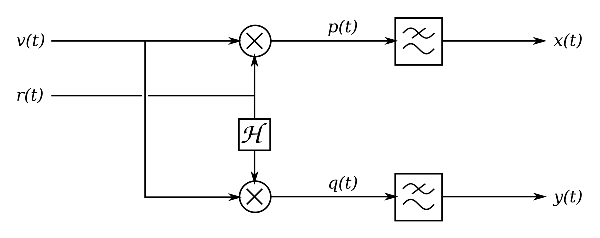
\includegraphics[width=\linewidth]{Images/lockin_gral.eps}
	\caption{Una señal de entrada $v(t)$ es inyectada al lock in. Posterior a la demodulación coherente, se extrae la señal de interés $z(t)=x(t)+jy(t)$}
	\label{fig:lockin}
\end{figure}

La figura \ref{fig:lockin} presenta un circuito lock in típico. El bloque transformada de Hilbert para una referencia senoidal corresponde a un desfasaje de 90°. La señal de salida se obtiene en forma de parte real e imaginaria, pero típicamente se expresa en forma amplitud y fase

\begin{equation*}
	z(t) = x(t) + j y(t) = R(t) e ^{j\Phi(t)}
\end{equation*}\\[-1em]

Donde la amplitud y fase se obtienen de las ecuaciones

\begin{equation*}
	R(t) = \sqrt{x^2(t)+y^2(t)} \qquad \qquad \Phi(t) = \arctan\frac{y(t)}{x(t)}
\end{equation*}\\


Para comprender el comportamiento esperando del demodulador coherente resulta útil visualizar las señales involucradas en el dominio de la frecuencia, análisis que se realiza en la figura \ref{fig:sigs_fourier}.

\begin{figure}[H]
	\centering
	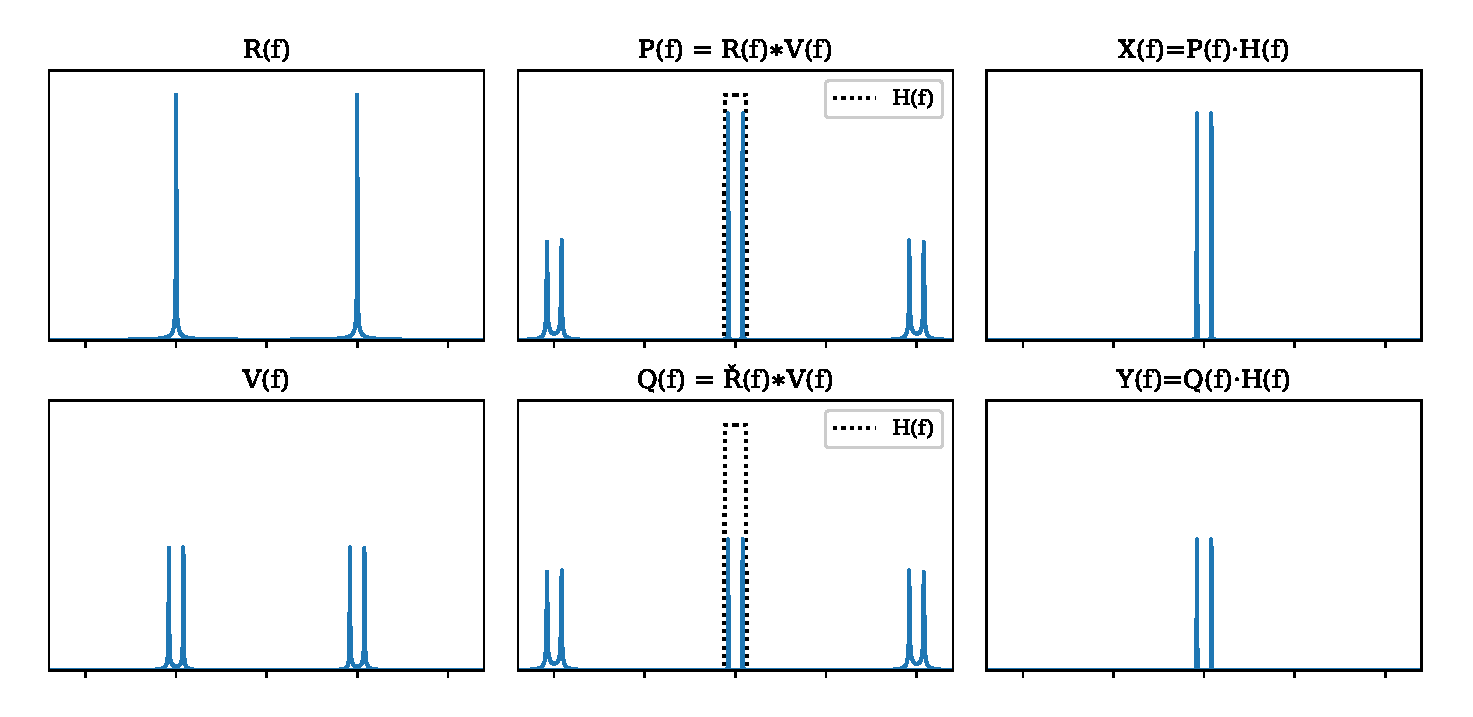
\includegraphics[width=\linewidth]{Images/sigs_fourier.eps}
	\caption{Realización en ausencia de ruido de las señales presentes en la figura \ref{fig:lockin} representadas en el dominio de la frecuencia, incluida la respuesta en frecuencia del filtro.}
	\label{fig:sigs_fourier}
\end{figure}

La salida $z(t)$ del demodulador coherente se puede interpretar como la entrada $v(t)$ transportada a banda base. Por este motivo la frecuencia de corte del filtro pasa bajos se debe elegir tal que acepte el ancho de banda de la señal a medir.

\section{Implementación}

La aplicación del amplificador lock in correspondiente a la práctica realizada es de medición de impedancias. Esto se realiza midiendo la transferencia de un circuito divisor de tensión con una impedancia incógnita.

\begin{figure}[H]
	\centering
	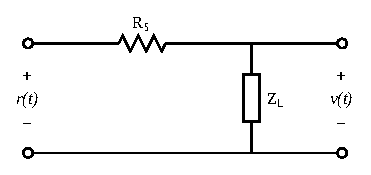
\includegraphics[width=0.75\linewidth]{Images/transferencia.eps}
	\caption{Circuito a medir, $R_S$ es una resistencia de valor conocido, y $Z_L$ una impedancia supuesta incógnita.}
	\label{fig:transferencia}
\end{figure}

En estas condiciones, se mide 
\begin{equation}
	H = \frac{v(t)}{r(t)} = \frac{Z}{R + Z} \quad \longrightarrow \quad Z =  \frac{HR}{1-H}	
\end{equation}

La relación $v(t) = H r(t)$ con $H \in \mathbb C$ implica que el ancho de banda de la señal a medir puede considerarse arbitrariamente chico.\\

El filtro elegido fue un FIR por su facilidad de implemntación y diseño respecto al IIR.\cite{haykin_8}
\begin{itemize}
	\item Al no tener polos en su función de transferencia, un FIR es siempre estable.
	\item La respuesta es de fase constante lo, cual permite conocer su retardo de grupo según la ecuación

	\begin{equation}\label{eq:tau}
		\tau = \frac{N-1}{2f_s}
	\end{equation}
	\item La aplicación de un FIR de respuesta al impulso $h$ a una señal $x$ es un único producto interno
	\begin{equation}\label{eq:fir}
		y_i = \sum_{j=0}^N h_jx_{i-j}= 
		\begin{bmatrix}
			x_i & \cdots & x_{i-N}
		\end{bmatrix}
		\begin{bmatrix}
			h_0 \\ \vdots \\ h_N	
		\end{bmatrix}
	\end{equation}
\end{itemize} 


Conociendo el valor de $\tau$ se decide a partir de que instante registrar valores tal de medir únicamente en régimen estacionario. Se elije la convención de que el régimen estacionario empieza a $t \ge 5\tau$.\\


Ya que lo que interesa medir en nuestro circuito es transferencia, resulta útil normalizar los valores medidos. Normalizando se independiza la medición de la tensión de alimentación del circuito y se mide transferencia diréctamente. El lock in implementado corresponde a la figura \ref{fig:nuestro_lockin}

\begin{figure}[H]
	\centering
	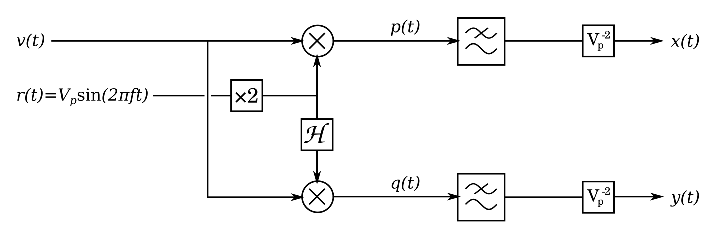
\includegraphics[width=\linewidth]{Images/nuestro_lockin.eps}
	\caption{Lock In implmentado para medición de impedancias. El módulo $\times 2$ aplicado a la referencia contrarresta un efecto de la demodulación visto en la figura \ref{fig:sigs_fourier} donde la mitad de la amplitud de la señal de interés es transportada a alta frecuencia y filtrada.}
	\label{fig:nuestro_lockin}
\end{figure}

\section{Método Experimental}

En primer lugar se midió la frecuencia máxima de 
muestreo que permite el dispositivo de medición, esta es necesaria para diseñar los filtros digitales y para conocer la máxima frecuencia de señal que se puede medir.\\

\begin{figure}[H]
	\centering
	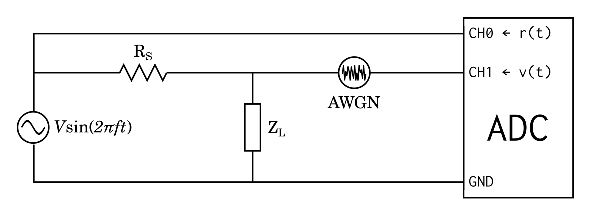
\includegraphics[width=\linewidth]{Images/circuito.eps}
	\caption{Circuito usado en el experimento. Los generadores de señal son RIGOL DG4102. El conversor analógico digital es Measurement Computing USB-1408FS.}
	\label{fig:circuito}
\end{figure}


Luego se ensambló el circuito de la figura 
\ref{fig:circuito}, en donde $ZL$ era de carácter
 puramente resistivo, y se pudo obtener 
el valor de la resistencia de carga $RL = ZL$ para 
comprobar el funcionamiento del lock in en el caso 
de impedancias reales.\\ 

Se utilizaron dos generadores de señal RIGOL DG4102 
para poder generar la señal de referencia y el ruido.
Para sumar éstas dos señales se tuvo que "flotar" la 
tierra de uno de los generadores dado que éstos no poseen 
tierra propia, sino que utilizan la de la red eléctrica.\\

Para la realización del lock in se implementó un 
script en python como se puede ver en el apéndice.
En el código se importó la librería del dispositivo 
de medición, el 
conversor analógico dígital USB-1408FS de la línea 
MEASUREMENT COMPUTING, para poder 
calibrarlo y realizar las mediciones.\\

Se implementaron 
las etapas de la figura \ref{fig:nuestro_lockin},
 en donde se optó por utilizar filtros FIR dada 
 su versatilidad y sencillez de implementación.\\

El programa toma la señal $v(t)$
y la normaliza utilizando su máximo valor de amplitud,
 siendo ésta la tensión de referencia. Además se mide 
 la señal $r(t)$ y se le aumenta la amplitud en un factor
 de 2 por el desarrollo que se necesita [Apéndice].
Se genera la señal $p(t)$ mediante la multiplicación de 
las dos señales tomadas.
Luego se genera la señal $q(t)$ desfasando 90◦
la señal 
mediante la transformada de Hilbert.
Por último se aplican filtros pasa bajos,
 obteniendo respectivamente las salidas $x(t)$ e $y(t)$,
  necesarias para obtener los
valores de amplitud y fase de la señal $v(t)$.


\section{Resultados}

Falta analizar que puntos usar de las gráficas y reportar
el valor $RL$ = (460±20)Ω, $C$ = (0.67±0.0.07)µF\\

Se determinó que la frecuencia máxima de muestreo es 
de aproximadamente 
500Hz, con una frecuencia máxima medible de 250Hz, 
según el teorema de muestreo de Nyquist. \cite{haykin_4}\\

Se midió el valor de $RL$ en función 
de la relación señal a ruido en la entrada para tres 
filtros FIR de distinto orden.
Se puede apreciar que el filto óptimo es el de mayor 
orden, dado que se utilizan mayor cantidad de 
mediciones para generar las señales medidas.

\begin{figure}[H]
	\centering
	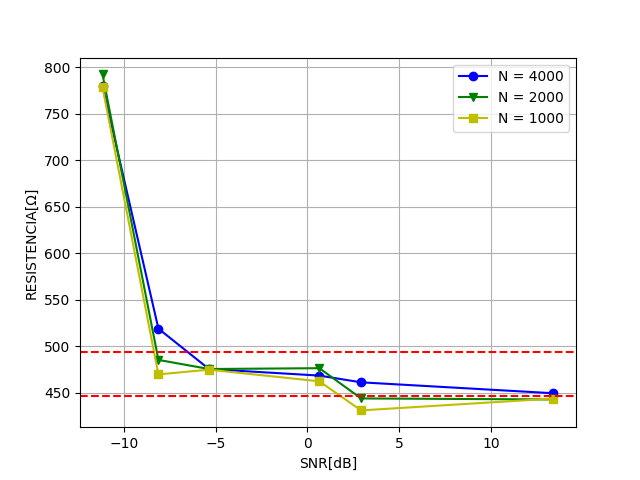
\includegraphics[width=\linewidth]{Images/RvsSNR(segunda).png}
	\caption{Resistencia de carga $RL$ obtenida con 
	el lock in en función
	de la relación señal ruido. Se obtuvo 
	$RL$ = (460±20)Ω.}
	\label{fig:RvsSNR}
\end{figure}

Para comprobar que el límite de funcionamiento 
del lock in no está limitado por el orden del 
filtro elegido sino por la SNR a la entrada
se realizaron distintas mediciones 
sobre el valor $RL$(dada la simpleza del circuito) 
para un valor de SNR a la entrada de -22.5dB para 
distintos filtros como se explaya en la figura 
\ref{fig:RORDEN}. Se aprecia un valor mas acercado 
al tabulado cuando se aumenta el orden del filtro, sin 
embargo está lejos de entrar en la cota del error 
tabulado, y ésto asegura que el limitante en éste 
lock in es el ruido a la entrada.\\

Cabe aclarar que los valores de resistencia que estamos
 midiendo están dos ordenes de magnitud por de 
 bajo de la impedancias de entrada del adc, y al estar en 
una conexión en paralelo predomina el valor de la resistencia 
que deseamos obtener.\\

\begin{figure}[H]
	\centering
	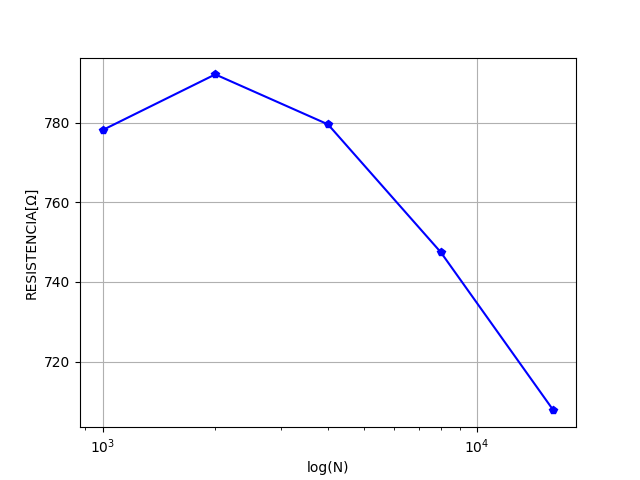
\includegraphics[width=\linewidth]{Images/RORDEN.png}
	\caption{Resistencia de carga $RL$ obtenida con 
	el lock in en función
	del orden del filtro empleado para  
	una relación señal ruido de -22.5dB}
	\label{fig:RORDEN}
\end{figure}

Por último se armó el circutio de la figura 
\ref{fig:CvsSNR} .Con ésto 
se midió el valor de la capacidad $CL$ para poder 
comprobar el funcionamiento del lock in en 
impedancias complejas.\\ 

\begin{figure}[H]
	\centering
	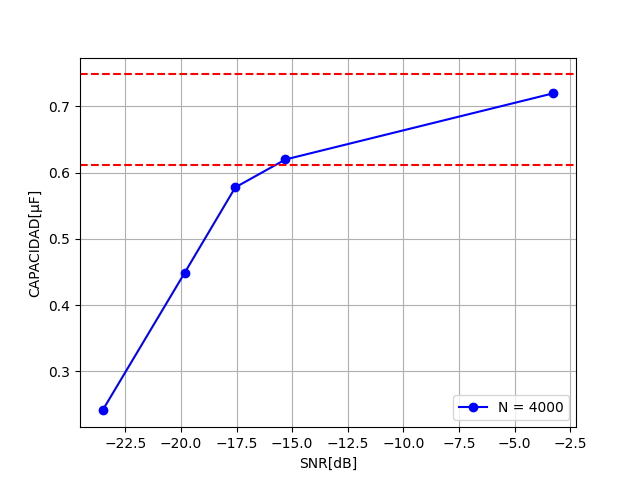
\includegraphics[width=\linewidth]{Images/CvsSNR(segunda).png}
	\caption{Capacidad de carga $C$ obtenida con 
	el lock in en función
	de la relación señal ruido. Se obtuvo 
	$C$ = (0.67±0.0.07)µF.}
	\label{fig:CvsSNR}
\end{figure}


\section{Discusión}
A la hora de implementar el lock in diseñado se tuvo 
la limitancia de un valor bajo en la frecuencia de 
muestreo máxima que permitía el adc utilizado, por lo 
que se sugiere renovar éste 
dispositivo para poder tener un mayor 
rango de funcionamiento.\\

Se recomienda no realizar mediciones 
en la que la frecuencia de referencia sea 
similar a la frecuencia de la red dado que 
ésto introduce un mayor nivel de ruido.


\section{Conclusiones}

Si bien los amplificadores lock in comerciales resuelven 
mediciones con SNR de 1:1000, es decir 60dB,
 se encuentra satisfactorio 
el rendimiento del lock in digital desarrollado, con 
una implementación relativamente sencilla.\\

Se concluye que la mínima SNR de entrada para el 
correcto funcionamiento del lock in implementado es de 
aproximadamente unos '-6dB por ejemplo'.

\bibliography{LockIn}
\bibliographystyle{plain}

\end{multicols}
\newpage
\begin{appendices}
\vspace{-1em}
\hrule
\vspace{1em}
\normalsize
\section{Apéndice 1 - Medición de SNR de Entrada}
\end{appendices}

\begin{multicols}{2}
\normalsize
A la entrada del lock in se mide $v(t) = s(t) + n(t)$. Es de interés para la práctica conocer la relación señal ruido, definida por la relación entre medias cuadráticas

\begin{equation}\label{eq:snr}
	SNR = \frac{E\left[s^2(t)\right]}{E\left[n^2\right(t)]}
\end{equation}\\[-1em]

Sin embargo, se desconocen las componentes individuales $s(t)$, $n(t)$ únicamente se conoce su suma y la frecuencia de $s(t)$.\\

Esto permite aproximar $s(t)$ y $n(t)$ usando filtros muy selectivos a frecuencia central $f_0$. Un filtro pasa banda para aproximar $s(t)$ y uno rechaza banda para aproximar $n(t)$, tal como indica la figura \ref{fig:circ_snr}.

\begin{figure}[H]
	\centering
	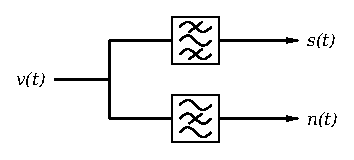
\includegraphics[width=0.75\linewidth]{Images/circ_snr.eps}
	\caption{Diagrama lógico de aproximación $s(t)$ y $n(t)$}
	\label{fig:circ_snr}
\end{figure}

Una realización de este proceso en el dominio de la frecuencia ante una medición de $v(t)$ se presenta en la figura \ref{fig:snr_filtros}

\begin{figure}[H]
	\centering
	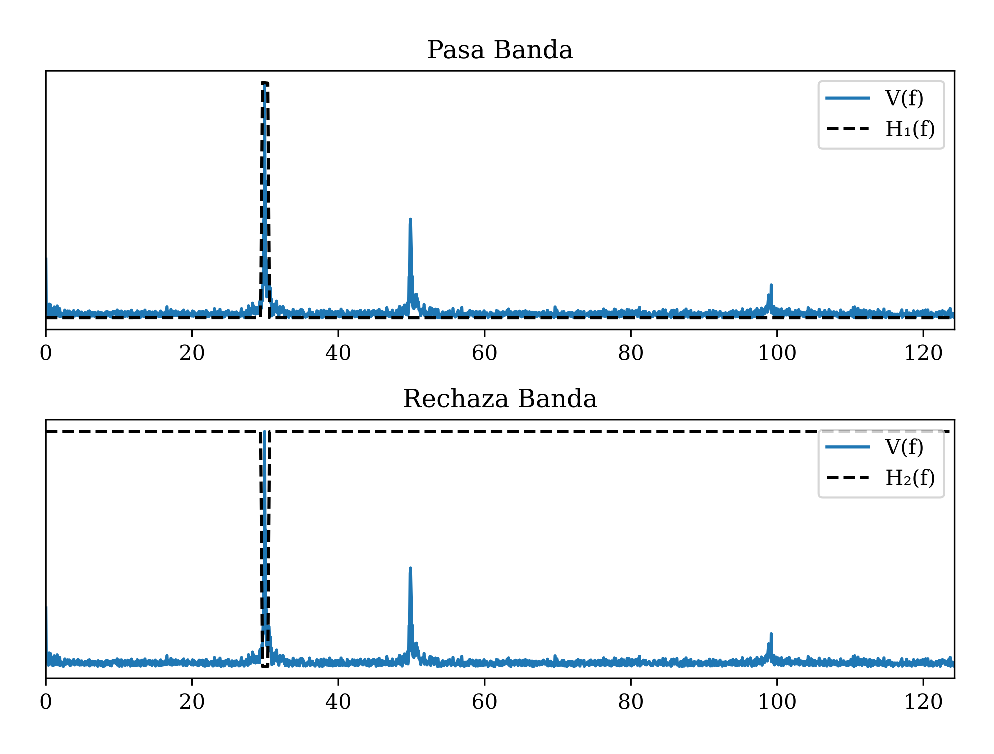
\includegraphics[width=\linewidth]{Images/snr_filtros.eps}
	\caption{Realización del circuito \ref{fig:circ_snr} en el dominio de la frecuencia.}
	\label{fig:snr_filtros}
\end{figure}

Resulta útil visualizar las señales en el dominio del tiempo para confirmar que el comportamiento del filtro es el esperado, la figura \ref{fig:snr_tiempo} es una realización del proceso con datos medidos experimentalmente.

\begin{figure}[H]
	\centering
	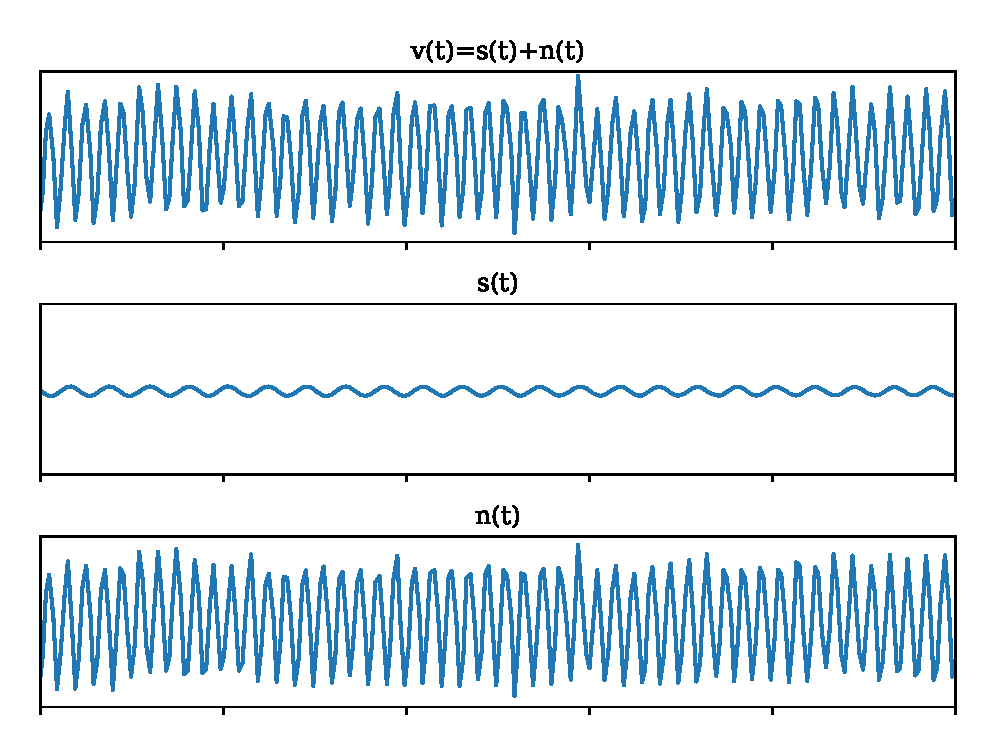
\includegraphics[width=\linewidth]{Images/snr_tiempo.eps}
	\caption{Efecto de la aplicación del circuito \ref{fig:circ_snr} a una señal ruidosa.}
	\label{fig:snr_tiempo}
\end{figure}

Las señales resultantes son usadas en la ecuación \ref{eq:snr}, y el resultado se informa en dB según la expresión

\begin{equation}\label{eq:snr_db}
	SNR_{dB} = 20\log_{10}\frac{E\left[s^2(t)\right]}{E\left[n^2\right(t)]}
\end{equation}

\end{multicols}

\end{document}
